\chapter{Opis projektnog zadatka}
		
		\section{Opseg projekta}
		
		Glavni je cilj razvoja aplikacije "Zamjena sobe" svim studentima koji su tijekom studiranja smješteni u studentskim domovina ponuditi rješenje za dva najveća problema s kojima se susreću. To su traženje sobe, to jest osobe za zamjenu te sam proces prijave te zamjene u Studentskim centrima.\\
		Nakon provedenog postupka natječaja za smještaj i objave liste ostvarenja prava na studentski smještaj, studenti imaju mogućnost zamjene doma ili sobe unutar dodijeljenog doma. 
		Studenti potencijalne zamjene traže uglavnom nasumično, usmenim putem ili putem raznih foruma i društvenih mreža, na posebnim grupama za pojedine gradove i studentske domove. Ovakvim izuzetno nepraktičnim i nestrukturiranim načinom zamjene vrlo je lako da se dva, moguće idealna oglasa, nikada ne povežu. Također, studentima se ne omogućuje postavljanje i traženje zamjene po više željenih kriterija.\\ 
		Ova bi aplikacija bila dostupna svima, ne samo studentima na određenom fakultetu ili gradu. Neregistrirani korisnik ima mogućnost pregleda svih oglasa i glavnih informacija o pojedinom oglasu: ime, prezime i profilna slika osobe koja je predala oglas, grad, paviljon i broj ponuđene sobe te željene kriterije nove sobe. Za korištenje svih ostalih funkcionalnosti neregistrirani korisnik može se registrirati, to jest stvoriti novi račun ili se prijaviti u sustav s već stvorenim računom. Kod prijave u sustav potrebno je upisati korisničko ime ili e-mail adresu i lozinku. Za registraciju korisnik mora upisati sljedeće podatke: 
		\begin{itemize}
			\item ime
			\item prezime
			\item korisničko ime
			\item e-mail adresa
			\item lozinka
			\item jmbag
		\end{itemize} 
		Prijavljenom korisniku omogućen je pregled njegova profila na kojemu može vidjeti i uređivati svoje osobne podatke i sliku profila, ili izbrisati svoj račun. Također, na pregledu "Moji oglasi" ima uvid u vlastite predane oglase koji mogu biti aktivni ili neaktivni. Aktivni oglas može dodatno uređivati ili ga učiniti neaktivnim.\\
		Kod predaje oglasa za zamjenu sobe student o sobi koju 'nudi' navodi sljedeće informacije:
		\begin{itemize}
			\item grad
			\item dom
			\item paviljon
			\item kat
			\item broj kreveta 
			\item tip kupaonice
		\end{itemize}
		Dodatno, student u tekstualno polje ima opciju upisa dodatnih značajki sobe, poput najbliže menze i slično. Osim informacija o svojoj sobi, student navodi i informacije o sobi koju želi, to jest željene kriterije. Jedino se ograničenje odnosi na grad - student ne može tražiti zamjenu u drugom gradu. Ostali kriteriji mogu biti i višestruki, na primjer može označiti da mu odgovaraju sobe s jednim, dva ili tri kreveta.\\
		Nakon što preda oglas, student ima uvid u ostale aktivne oglase koji odgovaraju njegovim željenim kriterijima. Ti oglasi mogu biti prikazani kao pojedinačni ili ulančani. Sve ponuđene oglase student može ocijeniti po stupnjevima podudaranja kriterija:
		\begin{itemize}
			\item 1 - sviđa mi se
			\item 2 - sviđa mi se jako
			\item 3 - to je to
			\item Ne prikazuj više ovaj oglas
		\end{itemize} 
		Osim pregleda ponuđenih oglasa, student također ima uvid u zaprimljene ponude za zamjenu - koji su studenti zainteresirani za njegov oglas te njihove oglase.\\
		Sustav periodički pretražuje nove dodane oglase i ažurira uparivanja po kriterijima. Kao što je već spomenuto, uz izravne, pojedinačne zamjene sustav nudi i potencijalne lance razmjene, ako takvi postoje.\\
		Nakon što oba studenta (ili svi studenti u slučaju lanca razmjene) ocijene razmjenu, sustav im šalje e-mail poruku kojom se traži da konačno potvrde zamjenu soba. Poveznica na određenu zamjenu sadržana je u e-mail poruci. \\
		Sve su potvrđene zamjene dostupne na uvid ovlaštenim djelatnicima pojedinog Studentskog centra. Nakon prijave u sustav zaključane zamjene izravno evidentiraju u sustavu Studentskog centra, bez potrebe za osobnom intervencijom studenata.
		
		\clearpage
		
		
		\section{Postojeća slična rješenja}
		
		Mnoga strana sveučilišta imaju slična rješenja za zamjenu soba, ali unutar svojih privatnih sustava koji su dostupni samo studentima toga sveučilišta. Jedan je takav primjer'Room Swap' sveučilišta \textit{The University of North Carolina at Chapel Hill}. 'Room Swap' je također dostupan samo studentima na sveučilištu 'North Carolina'. 
		Glavna je razlika između ovog sustava i naše aplikacije u tome što putem \textit{Room Swapa} student ne može provesti 'pravu' zamjenu sobe – može izabrati neku slobodnu sobu na kampusu ili sobu koja nije do kraja popunjena, ne može se direktno zamijeniti s drugom osobom, što bi naša aplikacija omogućavala.\\ 
		Student u sustavu \textit{Room Swap} prvo izabire zgradu te se klikom na zgradu otvara pregled katova i dostupnih slobodnih soba.
		
		\begin{figure}[H]
			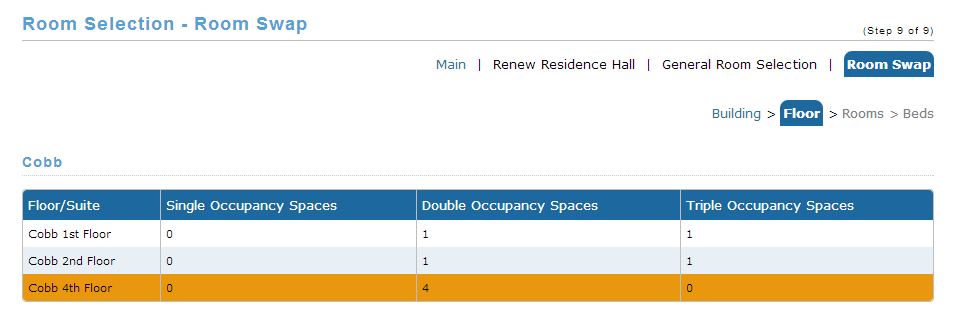
\includegraphics[width=.7\linewidth]{slike/rs8.png} %veličina u odnosu na širinu linije
			\centering
			\caption{Prikaz katova i dostupnih slobodnih soba na pojedinom katu}
			\label{fig:promjene} %label mora biti drugaciji za svaku sliku
		\end{figure}
	
		Još je jedna razlika u odnosu na našu aplikaciju to što nisu sve sobe dostupne svima. Na primjer, postoje 'First Year Experience Buildings' koje su dostupne samo brucošima. Također, sobe s više kreveta podijeljene su po spolu. 
		Nakon izbora kata aplikacija prikazuje tlocrt toga kata sa svim dostupnim sobama. 
		
		\begin{figure}[H]
			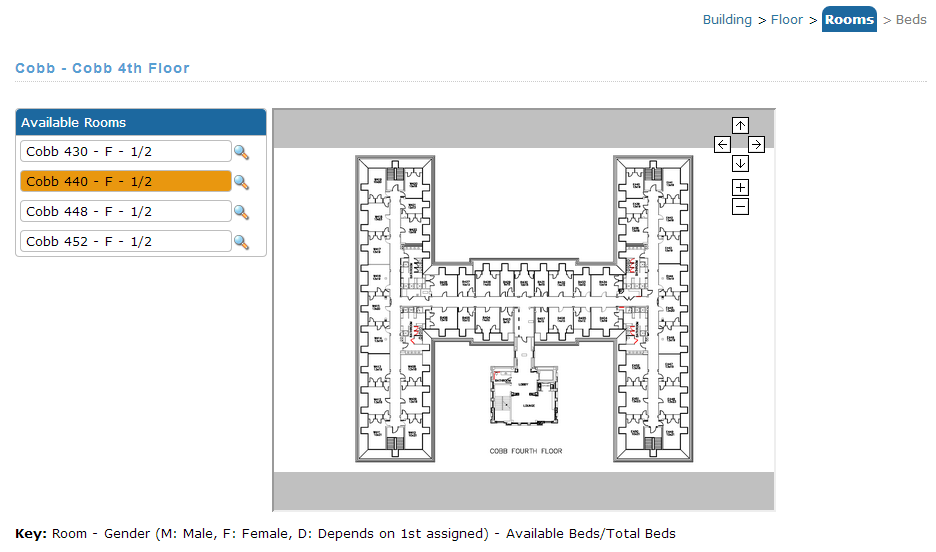
\includegraphics[scale=0.4]{slike/rs9.png} %veličina slike u odnosu na originalnu datoteku i pozicija slike
			\centering
			\caption{Tlocrt odabranog kata}
			\label{fig:promjene2}
		\end{figure}
	
		Klikom na sobu moguć je prikaz detalja o sobi ali i studentu kojemu je trenutno dodijeljena soba. Naša bi aplikacija, uz osnovne informacije o sobi poput doma, paviljona, kata i vrste, nudila i mogućnost detaljnijeg opisa - tip kupaonice, blizina menza itd. 
		
		\begin{figure}[H]
			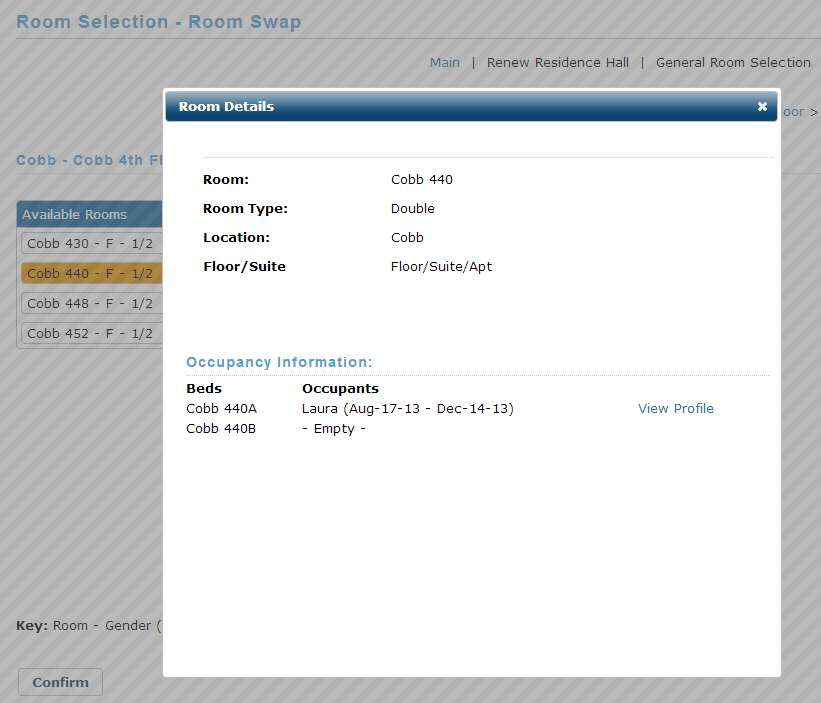
\includegraphics[scale=0.4]{slike/rs10.png} %veličina slike u odnosu na originalnu datoteku i pozicija slike
			\centering
			\caption{Detalji o sobi i studentima u sobi}
			\label{fig:promjene3}
		\end{figure}
	
		Nakon odabira sobe pokreće se odbrojavanje od 5 minuta unutar kojih student mora izabrati krevet u sobi i konačno potvrditi svoj potpuni odabir. Ako se odabir unutar 5 minuta ne potvrdi zamjena se neće provesti. Naša aplikacija ne bi postavljala vremensko ograničenje na potvrdu zamjene, već bi se čekala potvrda obje strane.
		
		\begin{figure}[H]
			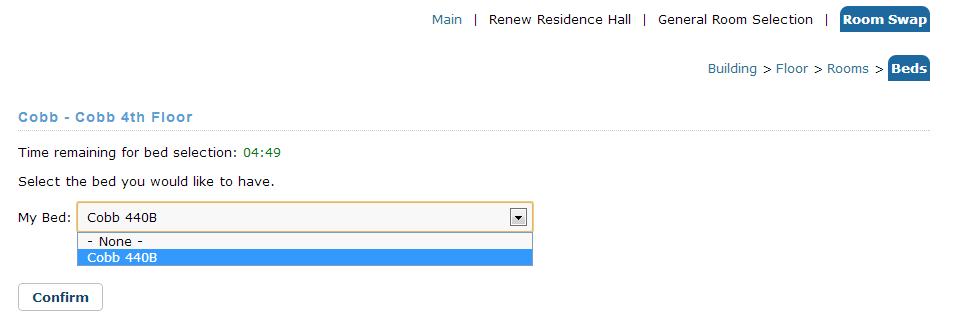
\includegraphics[scale=0.5]{slike/rs11.png} %veličina slike u odnosu na originalnu datoteku i pozicija slike
			\centering
			\caption{Odbrojavanje i konačni odabir}
			\label{fig:promjene4}
		\end{figure}
	
		\clearpage
		
		
		
		\eject
		
	